\section{Automated comments writing}
\subsection{Issues}
The following are the main issues we had to deal with concerning the documentation:
\begin{enumerate}
\item \textbf{Refactoring dependency}: It is impossible to put Doxygen tags and comments inside the code while we are working on the refactoring.
\item \textbf{Repetitive work}: The initial program contained 61 methods and 249 parameters to document. Mistakes in such work are difficult to avoid.
\item \textbf{Duplicate parameters} Most of the parameters are similar and it is important to keep coherence in the documentation by having the same description.
\item \textbf{Implemented functionalities} The quality of the documentation highly depends on the knowledge of the code we have.
\end{enumerate}
Here are the solutions we had for those problems:
\begin{enumerate}
\item[1-2] Automating the comment writing (see subsection \ref{auto})
\item[3] Adding an extra sheet for parameters (see subsection\ref{data})
\item[4] Having a deep look inside the code.
\end{enumerate}
\subsection{MySQL Database\label{data}}
The MySQL database is basically made to store the information on modules, routines and parameters from the Google Drive. We have 5 tables (see Figure \ref{table})
\begin{figure}[h!]
\begin{minipage}{0.45\textwidth}
\centering
\fbox{
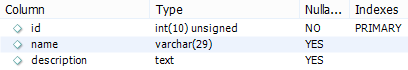
\includegraphics[width=\textwidth]{Image/docu-modules.png}
}
\fbox{
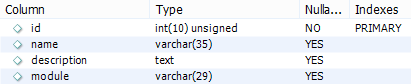
\includegraphics[width=\textwidth]{Image/docu-methods.png}
}
\fbox{
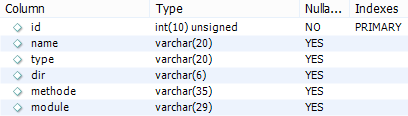
\includegraphics[width=\textwidth]{Image/docu-params.png}
}
\end{minipage}
\hfill
\begin{minipage}{0.5\textwidth}
\footnotesize
\begin{description}
\item[id] the key of each table
\item[name] the name of the module, method or parameter
\item[description] the description of the module, method or parameter
\item[module] the name of the module which the method belongs to
\item[type] the type of the parameter
\item[dir] the passing mode of the parameter
\item[method] the name of the method which the parameter belongs to
\end{description}
\end{minipage}
\caption{Description of the tables - From top to bottom: \textbf{modules}, \textbf{methods} and \textbf{parameters}\label{table}}
\end{figure}
\begin{itemize}
\item \textbf{modules}: classifies all the modules
\item \textbf{methods}: classifies all the routines
\item \textbf{parameters}: classifies all the parameters
\item \textbf{desc\_param}: classifies parameters whithout duplicate
\end{itemize}
Each Google sheet is copied locally using Microsoft Excel$^\copyright$ and registerd into CSV format. Thus, three files are produced: one for modules, one for methods and one for parameters. Then, a simple analysis is performed in order to fill the \textit{desc\_param} table with all the parameters without duplicate based on the name and the type. Finally, the result are written back into a dedicated sheet of the Google Drive.\\

As long as the refactoring evolves, we keept regularly the database up-to-date. Especially for the renaming of the modules, methods and parameters\footnote{cf section \ref{auto}}. And because the classifying does not take into account the reordering of the parameters\footnote{cf section \ref{reor}}, we added the table \textbf{type\_order} that put a "weight" on each type according to the refactoring.

\subsection{\textit{AutoComment} software\label{auto}}
This small software is the best solution we found to respond to repetitive work issues. This program in Java automatically write headers before each module and method by reading the Fortran files, extracting information from the database and write them back into target files in an other directory. We summed up its algorithm (see Algorithm \ref{algo}). 
\begin{algorithm}
\caption{\textit{AutoComment} algorithm}
\label{algo}
\begin{algorithmic}
\State Extract modules from the database
\ForAll{module in modules}
\State Open the corresponding file
\State Create a target file
\State Write header for the module in the target file
	\ForAll{line in file lines}
		\If{It is a comment line before a routine}
			\State Go to the next line
		\ElsIf{It is a routine declaration}
			\State Extract information on the routine from database
			\State Write header for the routine to the target file
		\Else
			\State Write the line in the target file
		\EndIf
	\EndFor
\EndFor
\end{algorithmic}
\end{algorithm}

The program is intend to be launched after the refactoring process. The key idea of this program is that we do not have to write the descriptions twice and we can work on refactoring and documentation at the same time. The algorithm is not fully explained as all the descriptions are not extracted from the database. Methods required advanced description and sometimes references and/or notes. It appeared that it is difficult to format long description in Excel sheets. Because we do not want too long comment lines, we used escape caracters but it is not well handled.  Besides the use of specific tag for such descriptions (@details, @see, @note) leads to some problem of integration in the database. That is why we choose to put further description of methods into separate text files named as the corresponding methods.
\section{Autogeneration with Doxygen}
\subsection{Doxygen tool parameters}
\subsection{Call and caller graphs}